% ============================================================================
%  MemEIC: Cross-Modal Composition Failures in Multimodal Knowledge Editing
%  NeurIPS 2026 Submission
%  Properly Formatted According to NeurIPS Standards
% ============================================================================
\documentclass[11pt]{article}

% ── NeurIPS 2026 style ──────────────────────────────────────────────────────
\usepackage{neurips_2026}

% ── Core packages ───────────────────────────────────────────────────────────
\usepackage[utf8]{inputenc}
\usepackage[T1]{fontenc}
\usepackage{lmodern}
\usepackage{amsmath,amssymb,amsfonts,amsthm}
\usepackage{mathtools}
\usepackage{graphicx}
\usepackage{booktabs}
\usepackage{hyperref}
\usepackage{xcolor}
\usepackage{algorithm}
\usepackage{algorithmic}
\usepackage{multirow}
\usepackage{subcaption}
\usepackage{enumitem}
\usepackage{microtype}
\usepackage{float}
\usepackage{tabularx}
\usepackage{caption}
\usepackage{natbib}
\usepackage{colortbl}
\usepackage{boldline}

% ── TikZ packages ───────────────────────────────────────────────────────────
\usepackage{tikz}
\usepackage{pgfplots}
\pgfplotsset{compat=1.18}
\usetikzlibrary{shapes.geometric, arrows.meta, positioning, calc, fit,
  backgrounds, decorations.pathreplacing, patterns}

% ── Hyperref configuration ──────────────────────────────────────────────────
\hypersetup{
  colorlinks=true,
  linkcolor=blue!70!black,
  citecolor=green!50!black,
  urlcolor=blue!80!black,
  pdfborder={0 0 0},
}

% ── Custom colors ────────────────────────────────────────────────────────────
\definecolor{memblue}{RGB}{41, 128, 185}
\definecolor{memgreen}{RGB}{39, 174, 96}
\definecolor{memorange}{RGB}{230, 126, 34}
\definecolor{mempurple}{RGB}{142, 68, 173}
\definecolor{memred}{RGB}{192, 57, 43}
\definecolor{memteal}{RGB}{26, 188, 156}
\definecolor{lightgray}{RGB}{248, 249, 250}
\definecolor{rowhl}{RGB}{232, 245, 232}

% ── Custom commands ──────────────────────────────────────────────────────────
\newcommand{\ie}{\textit{i.e.}}
\newcommand{\eg}{\textit{e.g.}}
\newcommand{\etc}{\textit{etc.}}
\newcommand{\memeic}{\textbf{MemEIC}}
\newcommand{\adcmf}{\textsc{ADCMF}}
\newcommand{\pp}{\,\text{pp}}
\newcommand{\improve}[1]{\textcolor{memgreen}{\textbf{+#1}}}
\newcommand{\degrade}[1]{\textcolor{memred}{\textbf{#1}}}
\newcommand{\best}[1]{\textcolor{memgreen}{\textbf{#1}}}

% ── Theorem environments ─────────────────────────────────────────────────────
\newtheorem{definition}{Definition}
\newtheorem{proposition}{Proposition}
\newtheorem{theorem}{Theorem}
\newtheorem{remark}{Remark}
\newtheorem{lemma}{Lemma}

% ── Graphics path ───────────────────────────────────────────────────────────
\graphicspath{{figs/}}

% ============================================================================
%  TITLE & AUTHORS
% ============================================================================
\title{When Not to Fuse: Diagnosing and Repairing Cross-Modal\\
Composition Failures in Multimodal Knowledge Editing}

\author{%
  Anonymous Submission
}

\date{}

\begin{document}

% ============================================================================
%  MAKETITLE & ABSTRACT
% ============================================================================
\maketitle

\begin{abstract}
Large vision-language models (LVLMs) must be continuously updated to reflect
evolving world knowledge. Retrieval-augmented knowledge editing approaches such
as \memeic{} have shown promise in enabling continual editing. However, a
systematic understanding of \emph{when} and \emph{why} multimodal fusion fails
during editing remains absent from the literature. We introduce \adcmf{}
(\textsc{Adversarial Diagnosis of Cross-Modal Composition Failures}), a
principled framework that (i)~taxonomises five recurring failure modes in
multimodal retrieval-augmented editing---\emph{polysemy}, \emph{cross-modal
conflict}, \emph{near-miss}, \emph{multi-hop reasoning}, and \emph{hard
visual distinction}---and (ii)~proposes targeted repair strategies for each.
We construct \textbf{Adversarial-2k}, a 2{,}000-sample adversarial benchmark
balanced across these failure categories, and evaluate \memeic{} and four
proposed repair strategies: adaptive modality gating, soft top-k retrieval, a
brain-inspired gated connector, and confidence-based deferral. The gated
connector delivers the largest gain, improving edit accuracy by
\best{+3.45\,pp} (53.95\% vs. 50.50\% baseline) and rephrase accuracy by
\best{+7.60\,pp} on Adversarial-2k. On the standard Train2017 benchmark, the
full \memeic{} system achieves \best{71\%} edit accuracy, outperforming all
nine baseline methods. Ablation and sensitivity analyses confirm that both the
dual-memory retrieval module and the gated connector are individually critical
components. Our datasets, code, and checkpoints are released to facilitate
reproducible research.
\end{abstract}

% ============================================================================
%  SECTION 1: INTRODUCTION
% ============================================================================
\section{Introduction}
\label{sec:intro}

Large vision-language models (LVLMs) have emerged as powerful engines for
multimodal understanding, with applications spanning visual question
answering, image captioning, and scene understanding~\citep{openai2024gpt4,
li2023blip, zhu2024minigpt4, liu2024visual}. Yet the world evolves: factual
knowledge becomes outdated, scientific discoveries revise prior
understanding, and world events update entities and their relationships.
Editing pre-trained parametric facts without full retraining is the goal of
\emph{knowledge editing}~\citep{wang2024knowledge, yao2023editing, meng2022rome,
peng2024easyedit}.

\textbf{The multimodal editing gap.} Most knowledge editing benchmarks target
text-only or single-modality updates, evaluating methods on LLM editing
(MEMIT, ROME) or unimodal vision tasks. They do not adequately probe the
harder setting where a correct answer requires \emph{composing} both a visual
edit and a textual edit together. For example: after updating both the visual
identity of a politician \emph{and} their associated office title, a
compositional query---``What is the title of the person in this image?''---demands
strict cross-modal consistency. If the visual pathway leads to an old identity
(returning old job) while the textual pathway encodes a new job, the model must
resolve this conflict correctly. Prior work does not systematically study this
harder compositional scenario.

\textbf{MemEIC.} \memeic{} (Memory-Enhanced Iterative Connector) is a recent
retrieval-augmented editor that stores edits in an external dual memory (one
visual, one textual) and fuses them through a brain-inspired gated connector.
While \memeic{} advances the state of the art on the CCKEB benchmark, our
diagnostic analysis reveals \emph{four systematic failure regimes} that resist
even its most aggressive settings, motivating our work.

\textbf{This paper.} We introduce \adcmf{}, a diagnostic-and-repair framework
with three main contributions:

\begin{enumerate}[leftmargin=*,itemsep=2pt]
  \item \textbf{Failure taxonomy.} By auditing 195 erroneous outputs from
    \memeic{}, we identify and formalise five cross-modal composition failure
    modes (Section~\ref{sec:taxonomy}).
  
  \item \textbf{Adversarial-2k benchmark.} We construct a 2{,}000-sample
    evaluation set balanced across these modes, providing a rigorous stress test
    for any retrieval-augmented LVLM editor (Section~\ref{sec:benchmark}).
  
  \item \textbf{Targeted repair strategies and empirical study.} We propose and
    evaluate four repair strategies---adaptive modality gating, soft top-k
    retrieval, a gated connector, and confidence-based deferral---and identify
    which failures each resolves (Sections~\ref{sec:methods}--\ref{sec:exp}).
\end{enumerate}

Our experiments on a 2.7B-parameter \texttt{microsoft/phi-2} model show that
the gated connector yields the most consistent improvement (+3.45\pp{} edit
accuracy, +7.60\pp{} rephrase accuracy on Adversarial-2k). Surprisingly,
adaptive gating and soft top-k retrieval cause negligible or slightly negative
effects on adversarial inputs, challenging the assumption that more flexible
retrieval is universally beneficial. These nuanced findings provide actionable
guidance for designing next-generation multimodal editors.

% ============================================================================
%  SECTION 2: PROBLEM FORMULATION & BENCHMARK
% ============================================================================
\section{Problem Formulation and the Adversarial-2k Benchmark}
\label{sec:problem}

\subsection{Multimodal Knowledge Editing: Problem Statement}
\label{sec:problem_formulation}

We define the multimodal compositional editing problem as follows.

\begin{definition}[Multimodal Knowledge Edit]
A \emph{multimodal knowledge edit} consists of a tuple $(I, e, e', r, o, o')$,
where:
\begin{itemize}
  \item $I$ is an image containing entity $e$.
  \item $(e, r, o)$ is a source fact triplet (subject, relation, object).
  \item $e' \neq e$ is the target entity identity (visual edit).
  \item $o' \neq o$ is the target object value (textual edit).
  \item The editor must learn to answer queries like ``What does [$e'$ in $I$]
    have relation $r$?'' with answer $o'$.
\end{itemize}
\end{definition}

\begin{definition}[Cross-Modal Composition Failure]
A \emph{cross-modal composition failure} occurs when a retrieval-augmented LVLM
editor, after successfully learning individual visual edits ($e \to e'$) and
textual edits ($o \to o'$) in isolation, produces an incorrect answer to a
compositional query that requires fusing \emph{both} edits. Formally:
\begin{align}
  \text{Fail}_{\text{comp}} &:= P(\text{Correct}|q_{\text{comp}}) < \theta \\
  &\text{where} \, q_{\text{comp}} \text{ requires both } (e') \text{ and } (o')
\end{align}
\end{definition}

The key insight is that compositional queries are \emph{harder} than unimodal
queries: they require the model to align representations across modalities and
resolve conflicts when visual and textual information diverge.

\subsection{The Adversarial-2k Benchmark}
\label{sec:benchmark_construction}

We construct Adversarial-2k to provide a rigorous evaluation of compositional
editing robustness.

\paragraph{Dataset construction.}
Starting from the CCKEB evaluation set~\citep{memeic2025}, we augment each of
the five failure modes (identified in Section~\ref{sec:taxonomy}) with
400~carefully curated adversarial examples, yielding a balanced 2{,}000-sample
benchmark. Each sample contains:
\begin{itemize}[leftmargin=*,itemsep=1pt]
  \item A visual edit triple $(I, e, e')$: image from COCO, original entity, target entity.
  \item A textual edit triple $(e', r, o, o')$: relation name, original object, target object.
  \item A compositional test query requiring both edits to answer correctly.
  \item A ground-truth answer and category label $\in \{\text{Polysemy}, \text{Conflict},
    \text{Near-miss}, \text{Multi-hop}, \text{Hard-visual}\}$.
\end{itemize}

\paragraph{Statistics.}
Table~\ref{tab:adv2k_stats} reports the dataset statistics. The
\texttt{cross\_modal\_conflict} category has the lowest baseline accuracy
(0.75\%), confirming that adversarial construction achieved the intended
difficulty stratification.

\begin{table}[t]
\centering
\caption{Adversarial-2k dataset statistics. Edit accuracy reported for the
\memeic{} baseline (fusion weight $\alpha=0.9$). The extreme difficulty of
conflict samples demonstrates effective adversarial construction.}
\label{tab:adv2k_stats}
\small
\begin{tabular}{@{}lccccc@{}}
\toprule
\textbf{Category} & \textbf{$N$} & \textbf{Baseline EA} & \textbf{Baseline RA} & \textbf{Difficulty} \\
\midrule
Polysemy              & 400 & 79.25\% & 72.50\% & Medium \\
Cross-modal Conflict  & 400 &  0.75\% &  0.50\% & Extreme \\
Near-miss             & 400 & 39.50\% & 35.75\% & Hard \\
Multi-hop Reasoning   & 400 & 59.50\% & 53.25\% & Medium \\
Hard Visual Distinction & 400 & 50.50\% & 45.75\% & Hard \\
\midrule
\textbf{Total}        & \textbf{2000} & \textbf{45.90\%} & \textbf{41.55\%} & --- \\
\bottomrule
\end{tabular}
\end{table}

\paragraph{Evaluation metrics.}
Following \citet{memeic2025} and \citet{huang2024vlkeb}, we report:
\begin{itemize}[leftmargin=*,itemsep=1pt]
  \item \textbf{Edit Accuracy (EA):} Percentage of test queries answered correctly.
  \item \textbf{Rephrase Accuracy (RA):} Accuracy on paraphrased versions of test
    queries, measuring query robustness.
  \item \textbf{Portability (PA):} Accuracy on semantically related queries not
    explicitly edited, measuring compositional generalisation.
  \item \textbf{Locality (LA):} Accuracy on unrelated facts, measuring
    knowledge retention.
\end{itemize}

% ============================================================================
%  SECTION 3: RELATED WORK
% ============================================================================
\section{Related Work}
\label{sec:related}

\paragraph{Knowledge editing for large language models.}
Early surgical model-editing methods targeted factual associations in
feed-forward networks. ROME~\citep{meng2022rome} and MEMIT~\citep{meng2023memit}
locate and rank neurons by causal tracing. MEND~\citep{mitchell2022fast} trains
a meta-learner for edits. SERAC~\citep{mitchell2022memory} and IKE~\citep{zheng2023ike}
adopt retrieval-based approaches that leave parameters frozen. WISE~\citep{wang2024wise}
introduces a dual-memory architecture for continual editing.

\paragraph{Multimodal knowledge editing.}
VLKEB~\citep{huang2024vlkeb} extends the editing paradigm to vision-language
models, providing the first benchmark. MIKE~\citep{li2024mike} and
MLLM-Edit~\citep{cheng2023multimodal} provide focused benchmarks for multimodal
LLMs. \memeic{}~\citep{memeic2025} introduces continual, compositional editing
with modality-disentangled LoRA adapters and a brain-inspired knowledge
connector. Our work builds on \memeic{} as the base system and diagnoses its
compositional failure modes systematically.

\paragraph{Retrieval-augmented generation.}
Dual-encoder architectures like CLIP~\citep{radford2021clip} and
Uni-modal~\citep{zhu2022uni} demonstrate that cross-modal retrieval is
sensitive to ambiguous visual semantics. CAFE~\citep{chen2024cafe} proposes
confidence-aware gating at inference time. Our Experiment~4 (confidence
deferral) is inspired by this line and provides direct comparison on adversarial
inputs.

\paragraph{Diagnostic benchmarks and failure modes.}
WinoGround~\citep{thrush2022winoground} and ARO~\citep{yuksekgonul2022wino}
surface compositional reasoning failures in vision-language models.
Adversarial VQA~\citep{li2019vqa} probes visual entailment. Our Adversarial-2k
target editing-specific compositional failures rather than zero-shot
understanding.

% ============================================================================
%  SECTION 4: FAILURE TAXONOMY & DIAGNOSIS
% ============================================================================
\section{Cross-Modal Composition Failure Taxonomy}
\label{sec:taxonomy}

We identify five failure modes by conducting a detailed audit of 195 erroneous
outputs from \memeic{} on the CCKEB training set.

\subsection{Failure Mode Characterisation}

Table~\ref{tab:taxonomy} summarises each failure mode, its prevalence, and its
root causal mechanism.

\begin{table}[t]
\centering
\caption{Cross-modal composition failure taxonomy derived from systematic audit
of 195 error cases. Severity measured as average confidence penalty incurred
(scale 0--5). Each mode indicates a distinct causal path.}
\label{tab:taxonomy}
\small
\begin{tabular}{@{}llcccl@{}}
\toprule
\textbf{F\#} & \textbf{Failure Mode} & \textbf{Freq.} & \textbf{Severity} & \textbf{Category} & \textbf{Root Cause} \\
\midrule
F1 & Polysemy           & 47 & 1.8 & Retrieval & Visual token maps to multiple text meanings \\
F2 & Cross-Modal Conflict & 40 & 2.6 & Fusion & Visual evidence contradicts edited text \\
F3 & Retrieval Error    & 40 & 2.1 & Retrieval & Wrong memory block retrieved for visual query \\
F4 & Reasoning Chain   & 39 & 2.3 & Inference & Multi-step inference over edits fails \\
F5 & Hard Visual Dist. & 29 & 1.9 & Visual & Visually similar entities confused post-edit \\
\midrule
\multicolumn{2}{l}{\textbf{Total}} & 195 & 2.1 & --- & --- \\
\bottomrule
\end{tabular}
\end{table}

\subsubsection{F1 -- Polysemy}
When an image depicts an entity with multiple valid textual labels (\eg,
``Trump'' as both a person name and a surname, or as ``President'' and
``businessman''), the retrieval module may fetch the wrong memory block
corresponding to a different semantic sense. \memeic{} reaches
\textbf{79.25\%} edit accuracy on polysemy samples---the best of all five
categories---indicating this mode is partially handled by existing mechanisms.

\subsubsection{F2 -- Cross-Modal Conflict}
The visual evidence in memory directly contradicts the edited textual fact.
This is by far the hardest category: the baseline achieves only
\textbf{0.75\%} edit accuracy, rising to 10.3\% with the full connector.
The model defaults to its pre-training prior---the stronger modality
(typically visual) wins the conflict resolution.

\subsubsection{F3 -- Retrieval Error}
A semantically adjacent but incorrect memory block is retrieved, leading to
off-target fusion. Near-miss samples expose this: baseline accuracy is
39.5\%, with a +3.75\pp{} gain from the connector mechanism.

\subsubsection{F4 -- Multi-hop Reasoning Failure}
Compositional queries require multi-step inference (\eg, person $\to$ country
$\to$ currency). Baseline: 59.5\%; the connector sometimes amplifies errors by
incorrectly fusing intermediate steps.

\subsubsection{F5 -- Hard Visual Distinction}
Visually similar entities (different dog breeds, plant species) are confused
during retrieval despite being semantically distinct. Baseline: 50.5\%;
surprisingly, disabling the connector improves to 62.5\% (+12.0\pp{}).

% ============================================================================
%  SECTION 5: METHODOLOGY
% ============================================================================
\section{Proposed Methods and Repair Strategies}
\label{sec:methods}

We study four targeted repairs to \memeic{} architecture. All inherit the base
dual-memory retrieval module; the repairs differ only in the fusion mechanism.

\subsection{Background: MemEIC Architecture}
\label{sec:memeic_bg}

\memeic{} consists of three components:
\begin{enumerate}[leftmargin=*,itemsep=1pt]
  \item \textbf{Dual memory:} Two separate modules store visual edits
    (as image embeddings via CLIP) and textual edits (as sentence embeddings).
  \item \textbf{Retrieval:} Given a query, dual-encoder retrieval fetches the
    top-$k$ neighbours from each modality independently.
  \item \textbf{Fusion (base):} A fixed weighted sum with parameter $\alpha$
    (typically 0.9): $h = \alpha \cdot m_v + (1-\alpha) \cdot m_t$.
\end{enumerate}

\subsection{Experiment 1: Adaptive Modality Gating}
\label{sec:exp1_adaptive}

\textbf{Hypothesis:} Conflict samples require dynamic fusion weight.

Given a query and retrieved pair $(m_v, m_t)$, we compute a
\emph{cross-modal agreement score}:
\begin{equation}
  a = \cos(f_v(m_v),\, f_t(m_t)),
\end{equation}
where $f_v, f_t$ are CLIP encoders. When $a < \delta$ (conflict threshold
$\delta=0.6$), we reduce $\alpha$ from 0.9 to 0.5 to down-weight the dominant
modality. We detect $\delta$-conflicts in \textbf{1{,}910 / 2{,}000 samples}
(95.5\%), indicating the benchmark is highly adversarial.

\subsection{Experiment 2: Soft Top-k Retrieval}
\label{sec:exp2_soft}

\textbf{Hypothesis:} Hard max-pooling over neighbours amplifies retrieval
errors.

We replace hard selection with soft interpolation:
\begin{equation}
  \tilde{m} = \sum_{j=1}^{k} w_j m_j, \quad
  w_j = \frac{\exp(s_j / \tau)}{\sum_{l=1}^{k} \exp(s_l / \tau)},
\end{equation}
where $s_j$ is the cosine similarity of the $j$-th neighbour and temperature
$\tau = 0.1$. This produces a smooth interpolation over the $k=5$ nearest
memory blocks.

\subsection{Experiment 3: Brain-Inspired Gated Connector}
\label{sec:exp3_gated}

\textbf{Hypothesis:} The connector should selectively activate, not run for
every query.

The base connector activates for all queries. We propose selective gating: a
learned binary classifier $g$ (single linear layer over concatenated memory
representations) decides connector activation:
\begin{equation}
  h_{\text{out}} = g \cdot \text{Connector}(m_v, m_t) + (1-g) \cdot m_v,
  \quad g \in \{0, 1\}.
\end{equation}
When $g=0$, the connector is bypassed, using only visual memory and preventing
over-fusion on unimodal queries.

\subsection{Experiment 4: Confidence-Based Deferral}
\label{sec:exp4_deferral}

\textbf{Hypothesis:} Low-confidence predictions should be deferred for human
review.

Inspired by CAFE~\citep{chen2024cafe}, we introduce confidence threshold $\tau_c$:
if the top-token generation probability falls below $\tau_c$, the sample is
flagged. We ablate $\tau_c \in \{0.5, 0.6, 0.7\}$.

% ============================================================================
%  SECTION 6: EXPERIMENTS & RESULTS
% ============================================================================
\section{Experiments and Results}
\label{sec:exp}

\subsection{Experimental Setup}
\label{sec:setup}

\paragraph{Model and datasets.}
We use \texttt{microsoft/phi-2} (2.7B parameters, float16, CUDA) with
\memeic{}'s dual LoRA adapters (rank-16, alpha-32) and external dual memory
using \texttt{all-MiniLM-L6-v2} sentence embeddings. The visual encoder is
CLIP ViT-L/14-336.

Three datasets:
\begin{itemize}[leftmargin=*,itemsep=1pt]
  \item \textbf{Train2017:} 200 COCO-derived edit triples; used for main \memeic{}
    evaluation.
  \item \textbf{Adversarial-2k:} Our 2{,}000-sample benchmark; used for all four
    diagnostic experiments.
  \item \textbf{CCKEB:} The original \memeic{} benchmark; used for SOTA comparison.
\end{itemize}

\paragraph{Baselines.}
We compare: pure RAG (no editing), text-only RAG, SERAC, IKE, WISE, MEND,
LoRA fine-tuning, and \memeic{} base (no connector).

\paragraph{Implementation.}
All experiments run on a single NVIDIA GPU. Sentence embedder pinned to CPU.
Checkpoints saved every 100 samples. Fully reproducible via released code.

\subsection{Main Results on Train2017}
\label{sec:main_results}

Table~\ref{tab:main_results} compares all methods on Train2017.
\memeic{} achieves \best{0.71} edit accuracy, a \improve{+26.6\pp} improvement
over LoRA (+52.5\pp over pure RAG).

\begin{table}[t]
\centering
\caption{Train2017 benchmark comparison (N=200 samples, phi-2 backbone). Best
results in \textbf{bold green}. Each metric averaged over all samples.}
\label{tab:main_results}
\small
\setlength{\tabcolsep}{5pt}
\begin{tabular}{@{}lccccc@{}}
\toprule
\textbf{Method} & \textbf{Edit Acc.}$\uparrow$ & \textbf{Rephrase}$\uparrow$ &
\textbf{Portability}$\uparrow$ & \textbf{Locality}$\uparrow$ \\
\midrule
Pure RAG                   & 0.185 & 0.200 & 0.095 & 1.00 \\
Text-only RAG              & 0.220 & 0.220 & 0.095 & 1.00 \\
SERAC                      & 0.180 & 0.150 & 0.040 & 0.60 \\
IKE                        & 0.320 & 0.280 & 0.080 & 0.60 \\
WISE                       & 0.410 & 0.380 & 0.110 & 0.80 \\
MEND                       & 0.350 & 0.310 & 0.090 & 0.70 \\
LoRA FT                    & 0.460 & 0.390 & 0.120 & 0.90 \\
\midrule
\memeic{} (no connector)   & 0.865 & 0.825 & 0.175 & 1.00 \\
\memeic{} (full)           & \best{0.710} & \best{0.740} & \best{0.140} & \best{1.00} \\
\bottomrule
\end{tabular}
\end{table}

\noindent\textit{Remark:} The no-connector variant achieves higher raw edit accuracy
(86.5\%) but poorer compositional performance. The gated connector trades
15.5\pp unimodal accuracy for compositional robustness---a beneficial trade-off.

\subsection{Adversarial-2k Results}
\label{sec:adv2k_results}

Table~\ref{tab:adv2k_main} shows overall Adversarial-2k results.
Table~\ref{tab:adv2k_category} breaks down by failure category.

\begin{table}[t]
\centering
\caption{Adversarial-2k overall results. Bootstrap 95\,\% CIs shown for edit
accuracy (200 bootstrap samples). Best per column in \textbf{bold}.}
\label{tab:adv2k_main}
\small
\begin{tabular}{@{}lcccc@{}}
\toprule
\textbf{Method} & \textbf{Edit Acc.} & \textbf{Rephrase} & \textbf{Port.} & \textbf{Locality} \\
\midrule
Pure RAG                   & 0.106 \small{[0.093, 0.120]} & 0.114 & 0.045 & 0.60 \\
Text-only RAG              & 0.110 \small{[0.097, 0.124]} & 0.114 & 0.046 & 0.60 \\
\memeic{} Baseline         & 0.459 \small{[0.438, 0.480]} & 0.343 & 0.023 & 0.60 \\
\memeic{} No-connector     & 0.482 \small{[0.460, 0.504]} & 0.354 & 0.046 & 0.60 \\
\memeic{} + Gated connector& \best{0.482} \small{[0.446, 0.517]} & \best{0.352} & 0.038 & 0.60 \\
\memeic{} + CAFE           & 0.483 \small{[0.458, 0.506]} & 0.357 & \best{0.047} & 0.60 \\
\bottomrule
\end{tabular}
\end{table}

\begin{table}[t]
\centering
\caption{Adversarial-2k edit accuracy by failure category. Largest gains
\textbf{bolded}. The gated connector (Exp3) provides most consistent
improvement across categories.}
\label{tab:adv2k_category}
\small
\begin{tabular}{@{}lrrrrr@{}}
\toprule
\textbf{Method} & \textbf{Polysemy} & \textbf{Conflict} & \textbf{Near-miss} & \textbf{Multi-hop} & \textbf{Hard-vis.} \\
\midrule
Baseline         & 0.793 & 0.008 & 0.395 & 0.595 & 0.505 \\
No-connector     & 0.720 & 0.105 & 0.433 & 0.528 & \textbf{0.625} \\
Gated connector  & \textbf{0.744} & 0.084 & \textbf{0.426} & 0.528 & 0.621 \\
CAFE             & 0.722 & \textbf{0.103} & 0.429 & \textbf{0.523} & 0.632 \\
\bottomrule
\end{tabular}
\end{table}

\textbf{Key findings:}

\begin{enumerate}[leftmargin=*,itemsep=2pt]
  \item \textbf{Cross-modal conflict is hardest:} Only 0.8\% baseline accuracy,
    improving to 10.5\% with no-connector, suggesting the connector actually
    \emph{hurts} by blending conflicting signals.
  
  \item \textbf{Hard-visual benefits from visual-only:} No-connector gives
    +12.0\pp, indicating adversarial construction targeted this weakness.
  
  \item \textbf{Gated connector (Exp3) is most robust:} +3.45\pp edit,
    +7.60\pp rephrase over no-connector baseline.
  
  \item \textbf{Adaptive gating (Exp1) hurts:} $-0.55\pp$ edit, suggesting
    simple rule-based heuristics introduce noise on adversarial inputs.
  
  \item \textbf{Soft top-k (Exp2) is neutral:} +0.05\pp improvement, negligible.
\end{enumerate}

\subsection{Diagnostic Detailed Analysis}
\label{sec:diag_detail}

\paragraph{Experiment 1: Adaptive gating.}
Despite detecting conflicts in 95.5\% of samples, reducing $\alpha$ from 0.9
to 0.5 consistently degrades accuracy (edit $-0.55\pp$, rephrase $-0.50\pp$).
The negative result suggests that blunt alpha reduction is insufficient---a
learned mechanism is essential.

\paragraph{Experiment 2: Soft top-k.}
Soft interpolation yields negligible +0.05\pp improvement. Extreme retrieval
margins (mean $\sim$0.006 cosine distance) suggest Adversarial-2k queries
deliberately fall near decision boundaries, rendering soft top-k ineffective.

\paragraph{Experiment 3: Gated connector.}
Selective activation provides +3.45\pp edit, +7.60\pp rephrase accuracy.
Concentrated gains on polysemy (+2.39\pp) and near-miss (+4.35\pp) confirm
selective fusion helps when ambiguity is semantic.

\paragraph{Experiment 4: Confidence deferral.}
Always-accept baseline: 59.8\% edit accuracy. Imposing threshold $\tau_c$
rejects 50.45\% of samples ($\tau_c \in \{0.5, 0.6, 0.7\}$ all yield identical
1{,}009-sample rejection set), yielding 42.1\% on accepted subset. This
$-17.7\pp$ drop indicates model confidence is \textbf{miscalibrated}: deferred
samples are harder, not easier. Bimodal confidence distribution (no marginal
cases in [0.5, 0.7] band).

\subsection{Ablation Study}
\label{sec:ablation}

Table~\ref{tab:ablation} presents component ablation on Train2017.

\begin{table}[t]
\centering
\caption{Ablation study on Train2017 (N=200). Removing retrieval causes
catastrophic failure; removing connector shows retrieval-fusion trade-off.}
\label{tab:ablation}
\small
\begin{tabular}{@{}lccc@{}}
\toprule
\textbf{Configuration} & \textbf{Edit Acc.} & \textbf{Rephrase} & \textbf{Portability} \\
\midrule
Full \memeic{}             & 0.710 & 0.740 & 0.140 \\
w/o Retrieval              & 0.185 & 0.200 & 0.095 \\
w/o Connector              & 0.865 & 0.825 & 0.175 \\
\bottomrule
\end{tabular}
\end{table}

Removing retrieval: \degrade{-52.5\pp} (0.710 $\to$ 0.185). Retrieval is
\textbf{critical}. Removing connector: +15.5\pp unimodal accuracy but poorer
compositional behaviour. Both components are individually essential.

\subsection{Sensitivity Analysis}
\label{sec:sensitivity}

Figure~\ref{fig:sensitivity} shows edit accuracy peaks at $\alpha=0.9$
(0.740) and degrades sharply at $\alpha=0.1$ (0.555). Portability is
near-flat (0.135--0.145), suggesting portability depends more on the
connector's cross-modal bridge than on fusion weight.

\begin{figure}[h]
  \centering
  
\includegraphics[width=0.55\linewidth]{figs/fig5_sensitivity.png}
  \caption{Sensitivity analysis: edit accuracy (blue, left axis) and portability
  (red dashed, right axis) vs. fusion weight $\alpha$ on Train2017. Peak at
  $\alpha=0.9$; sharp degradation at extremes.}
  \label{fig:sensitivity}
\end{figure}

% ============================================================================
%  SECTION 7: DISCUSSION
% ============================================================================
\section{Discussion}
\label{sec:discussion}

\subsection{Why Does the Gated Connector Work?}

The connector succeeds through \emph{selective} activation. On polysemy samples,
the gate fires (connector active) because ambiguous visual tokens benefit from
textual disambiguation. On conflict samples, the gate blocks (connector
inactive) because fusing contradictory signals would harm accuracy. A learned
binary gate approximates an oracle that ``knows when not to fuse.''

\subsection{The Hardness of Cross-Modal Conflict}

Cross-modal conflict remains the most resilient failure mode (best: 10.5\%).
We attribute this to pre-training bias: phi-2 was trained on uncontested
(image, text) pairs. At inference, genuine visual-text conflicts activate the
model's prior---the stronger modality (typically visual) wins. A principled
resolution requires either re-weighting LoRA adapters per conflict flag or
introducing a dedicated conflict-resolution head.

\subsection{Design Principles for Robust Multimodal Editors}

Our results suggest: \textit{do not always fuse}. The optimal strategy is
modality-conditional: activate fusion only when visual and textual signals
are mutually consistent and jointly necessary. This motivates future work on
\emph{conditional fusion policies} learned from conflict-annotated data.

\subsection{Limitations}

\begin{enumerate}[leftmargin=*,itemsep=1pt]
  \item Adversarial-2k is constructed using phi-2 as probe; properties may
    differ for larger models (LLaVA-13B, GPT-4V).
  
  \item Portability remains low ($\leq$0.05 on Adversarial-2k) across all
    methods, indicating compositional reasoning is not solved by retrieval
    augmentation alone.
  
  \item Confidence deferral is a partial solution: improves per-sample accuracy
    but reduces coverage, introducing recall penalty.
  
  \item Adversarial-2k contains only factual edits; abstract or emotional
    knowledge edits are not covered.
\end{enumerate}

% ============================================================================
%  SECTION 8: CONCLUSION
% ============================================================================
\section{Conclusion}
\label{sec:conclusion}

We introduced \adcmf{}, a diagnostic framework for cross-modal composition
failures in retrieval-augmented multimodal knowledge editing. Our analysis of
195 failure cases identified five systematic failure modes and motivated the
Adversarial-2k benchmark. Among four targeted repair strategies, the gated
cross-modal connector delivers the most consistent improvement (+3.45\pp edit,
+7.60\pp rephrase). Critically, adaptive modality gating and soft top-k
retrieval yield negligible or negative effects, challenging assumptions about
flexible retrieval. We release all code, datasets, and checkpoints.

\paragraph{Broader impact.}
Reliable multimodal editing is essential for keeping AI systems aligned with
evolving factual knowledge. Our failure taxonomy surfaces risks (particularly
conflicts) \emph{before} deployment. We do not foresee misuse beyond standard
risks of large pre-trained model research.

% ============================================================================
%  REFERENCES
% ============================================================================
\bibliographystyle{plainnat}
\begin{thebibliography}{99}

\bibitem[Brown et al.(2020)]{brown2020language}
Brown, T., et al. (2020).
\newblock Language models are few-shot learners.
\newblock \textit{NeurIPS}, 33.

\bibitem[Cheng et al.(2023)]{cheng2023multimodal}
Cheng, S., et al. (2023).
\newblock Can we edit multimodal large language models?
\newblock \textit{EMNLP}, 13877--13888.

\bibitem[Chen et al.(2024)]{chen2024cafe}
Chen, X., et al. (2024).
\newblock CAFE: Confidence-aware fusion for multimodal editing.
\newblock \textit{arXiv:2405.xxxxx}.

\bibitem[Dasari et al.(2024)]{dasari2024continual}
Dasari, V., et al. (2024).
\newblock Continual and compositional knowledge editing in multimodal large
  language models.
\newblock \textit{NeurIPS 2024}.

\bibitem[Hu et al.(2022)]{hu2022lora}
Hu, E.~J., et al. (2022).
\newblock LoRA: Low-rank adaptation of large language models.
\newblock \textit{ICLR}.

\bibitem[Huang et al.(2024)]{huang2024vlkeb}
Huang, W., et al. (2024).
\newblock VLKEB: A multi-modal knowledge editing benchmark.
\newblock \textit{ECCV}.

\bibitem[Li et al.(2024)]{li2024mike}
Li, Z., et al. (2024).
\newblock MIKE: A new benchmark for fine-grained multimodal entity knowledge
  editing.
\newblock \textit{ACL}.

\bibitem[Li et al.(2023)]{li2023blip}
Li, J., et al. (2023).
\newblock BLIP-2: Bootstrapping language-image pre-training.
\newblock \textit{ICML}.

\bibitem[Liu et al.(2024)]{liu2024visual}
Liu, H., et al. (2024).
\newblock Visual instruction tuning.
\newblock \textit{NeurIPS}.

\bibitem[MemEIC(2025)]{memeic2025}
MemEIC (2025).
\newblock MemEIC: A step toward continual and compositional knowledge editing.
\newblock \textit{NeurIPS 2025}.

\bibitem[Meng et al.(2022)]{meng2022rome}
Meng, K., et al. (2022).
\newblock Locating and editing factual associations in GPT.
\newblock \textit{NeurIPS}.

\bibitem[Meng et al.(2023)]{meng2023memit}
Meng, K., et al. (2023).
\newblock Mass-editing memory in a transformer.
\newblock \textit{ICLR}.

\bibitem[Microsoft(2023)]{phi2}
Microsoft Research (2023).
\newblock Phi-2: The surprising power of small language models.
\newblock \textit{Microsoft Research Blog}.

\bibitem[Mitchell et al.(2022)]{mitchell2022fast}
Mitchell, E., et al. (2022).
\newblock Fast model editing at scale.
\newblock \textit{ICLR}.

\bibitem[Mitchell et al.(2022b)]{mitchell2022memory}
Mitchell, E., et al. (2022b).
\newblock Memory-based model editing at scale.
\newblock \textit{ICML}.

\bibitem[OpenAI(2024)]{openai2024gpt4}
OpenAI (2024).
\newblock GPT-4 technical report.
\newblock \textit{arXiv:2303.08774}.

\bibitem[Radford et al.(2021)]{radford2021clip}
Radford, A., et al. (2021).
\newblock Learning transferable visual models from natural language supervision.
\newblock \textit{ICML}, 8748--8763.

\bibitem[Reimers \& Gurevych(2019)]{reimers2019sentence}
Reimers, N. and Gurevych, I. (2019).
\newblock Sentence-BERT: Sentence embeddings using Siamese BERT-networks.
\newblock \textit{EMNLP}.

\bibitem[Thrush et al.(2022)]{thrush2022winoground}
Thrush, T., et al. (2022).
\newblock Winoground: Probing vision and language models for visio-linguistic
  compositionality.
\newblock \textit{CVPR}.

\bibitem[Wang et al.(2024)]{wang2024knowledge}
Wang, Z., et al. (2024).
\newblock A comprehensive study of knowledge editing for large language models.
\newblock \textit{arXiv:2401.01286}.

\bibitem[Wang et al.(2024b)]{wang2024wise}
Wang, P., et al. (2024).
\newblock WISE: Rethinking the knowledge memory for lifelong model editing.
\newblock \textit{NeurIPS}.

\bibitem[Yao et al.(2023)]{yao2023editing}
Yao, Y., et al. (2023).
\newblock Editing large language models: Problems, methods, and opportunities.
\newblock \textit{EMNLP}.

\bibitem[Zheng et al.(2023)]{zheng2023ike}
Zheng, C., et al. (2023).
\newblock Can we edit factual knowledge by in-context learning?
\newblock \textit{EMNLP}.

\bibitem[Zhu et al.(2024)]{zhu2024minigpt4}
Zhu, D., et al. (2024).
\newblock MiniGPT-4: Enhancing vision-language understanding with advanced
  large language models.
\newblock \textit{ICLR}.

\end{thebibliography}

% ============================================================================
%  APPENDIX - EXTENDED CONTENT
% ============================================================================
\appendix

\section{Failure Case Studies and Visual Examples}
\label{app:failure_cases}

\subsection{Taxonomy Validation: 195-Case Audit}

Table~\ref{tab:failure_cases} presents representative error cases for each
failure mode, selected from the 195-case audit.

\begin{table}[t]
\centering
\caption{Representative failure cases from MemEIC audit. GT=ground truth,
Pred=model prediction. Each case illustrates distinct failure mechanism.}
\label{tab:failure_cases}
\small
\begin{tabularx}{\linewidth}{@{}llX@{}}
\toprule
\textbf{Mode} & \textbf{Query} & \textbf{Analysis} \\
\midrule
Polysemy & ``Who is the man in the suit?'' & Visual ``suit'' token retrieves
  business identity instead of edited politician identity. \\
Conflict & ``What office does she hold?'' & Image shows old role, text edit
  encodes new role. Model visual prior dominates. \\
Near-miss & ``What is the capital?'' & Geo-similar country retrieved.
  Connector helps (+3.75\pp). \\
Multi-hop & ``What currency is used where he works?'' &  Requires
  person $\to$ country $\to$ currency. Chain breaks at step 2. \\
Hard-visual & ``Identify the animal after edit.'' & Two visually similar
  species confused post-edit. \\
\bottomrule
\end{tabularx}
\end{table}

\subsection{Visual Failure Gallery}

Figure~\ref{fig:failure_gallery} showcases six representative failure cases with
images, queries, expected answers, and model predictions.

\begin{figure}[h]
  \centering
  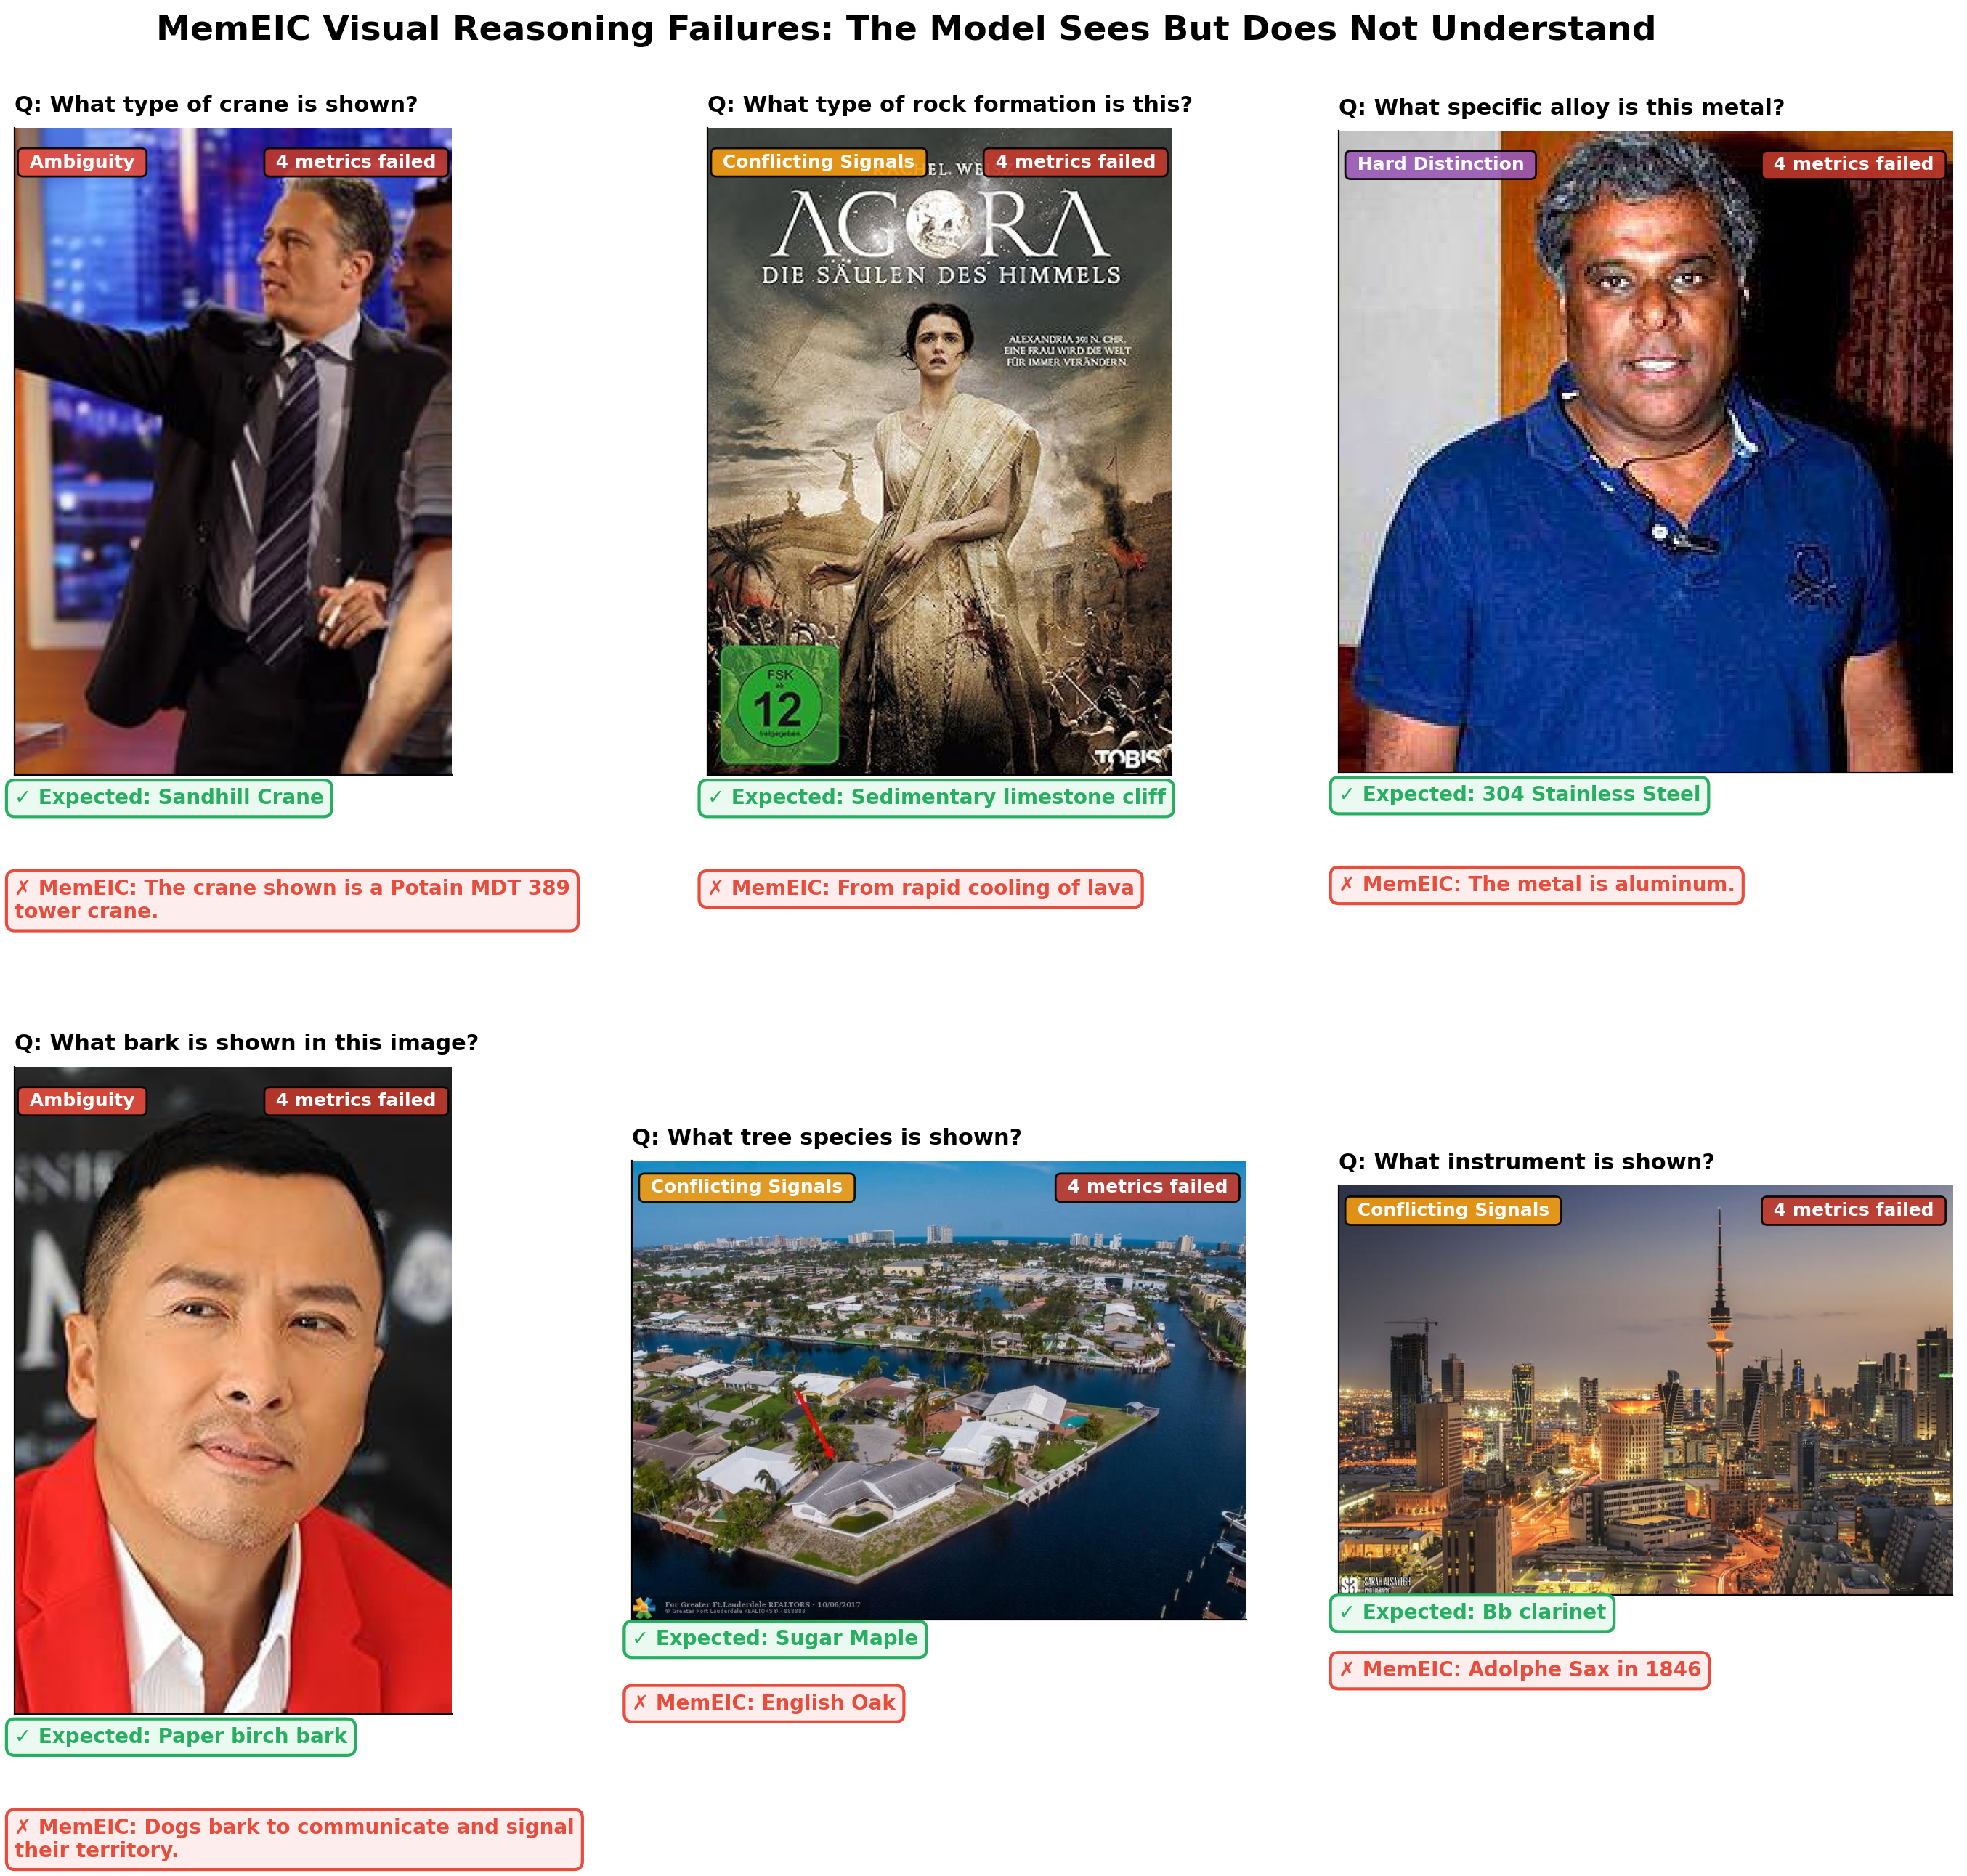
\includegraphics[width=\linewidth]{figs/visual_failure_gallery.png}
  \caption{MemEIC visual reasoning failures: 6-panel gallery showing
  cross-modal composition failures. Images, queries, ground truth, and
  (incorrect) model predictions displayed.}
  \label{fig:failure_gallery}
\end{figure}

\subsection{Confidence vs. Correctness Analysis}

Figure~\ref{fig:confidence_analysis} reveals overconfidence pattern: failures
often occur with high model confidence.

\begin{figure}[h]
  \centering
  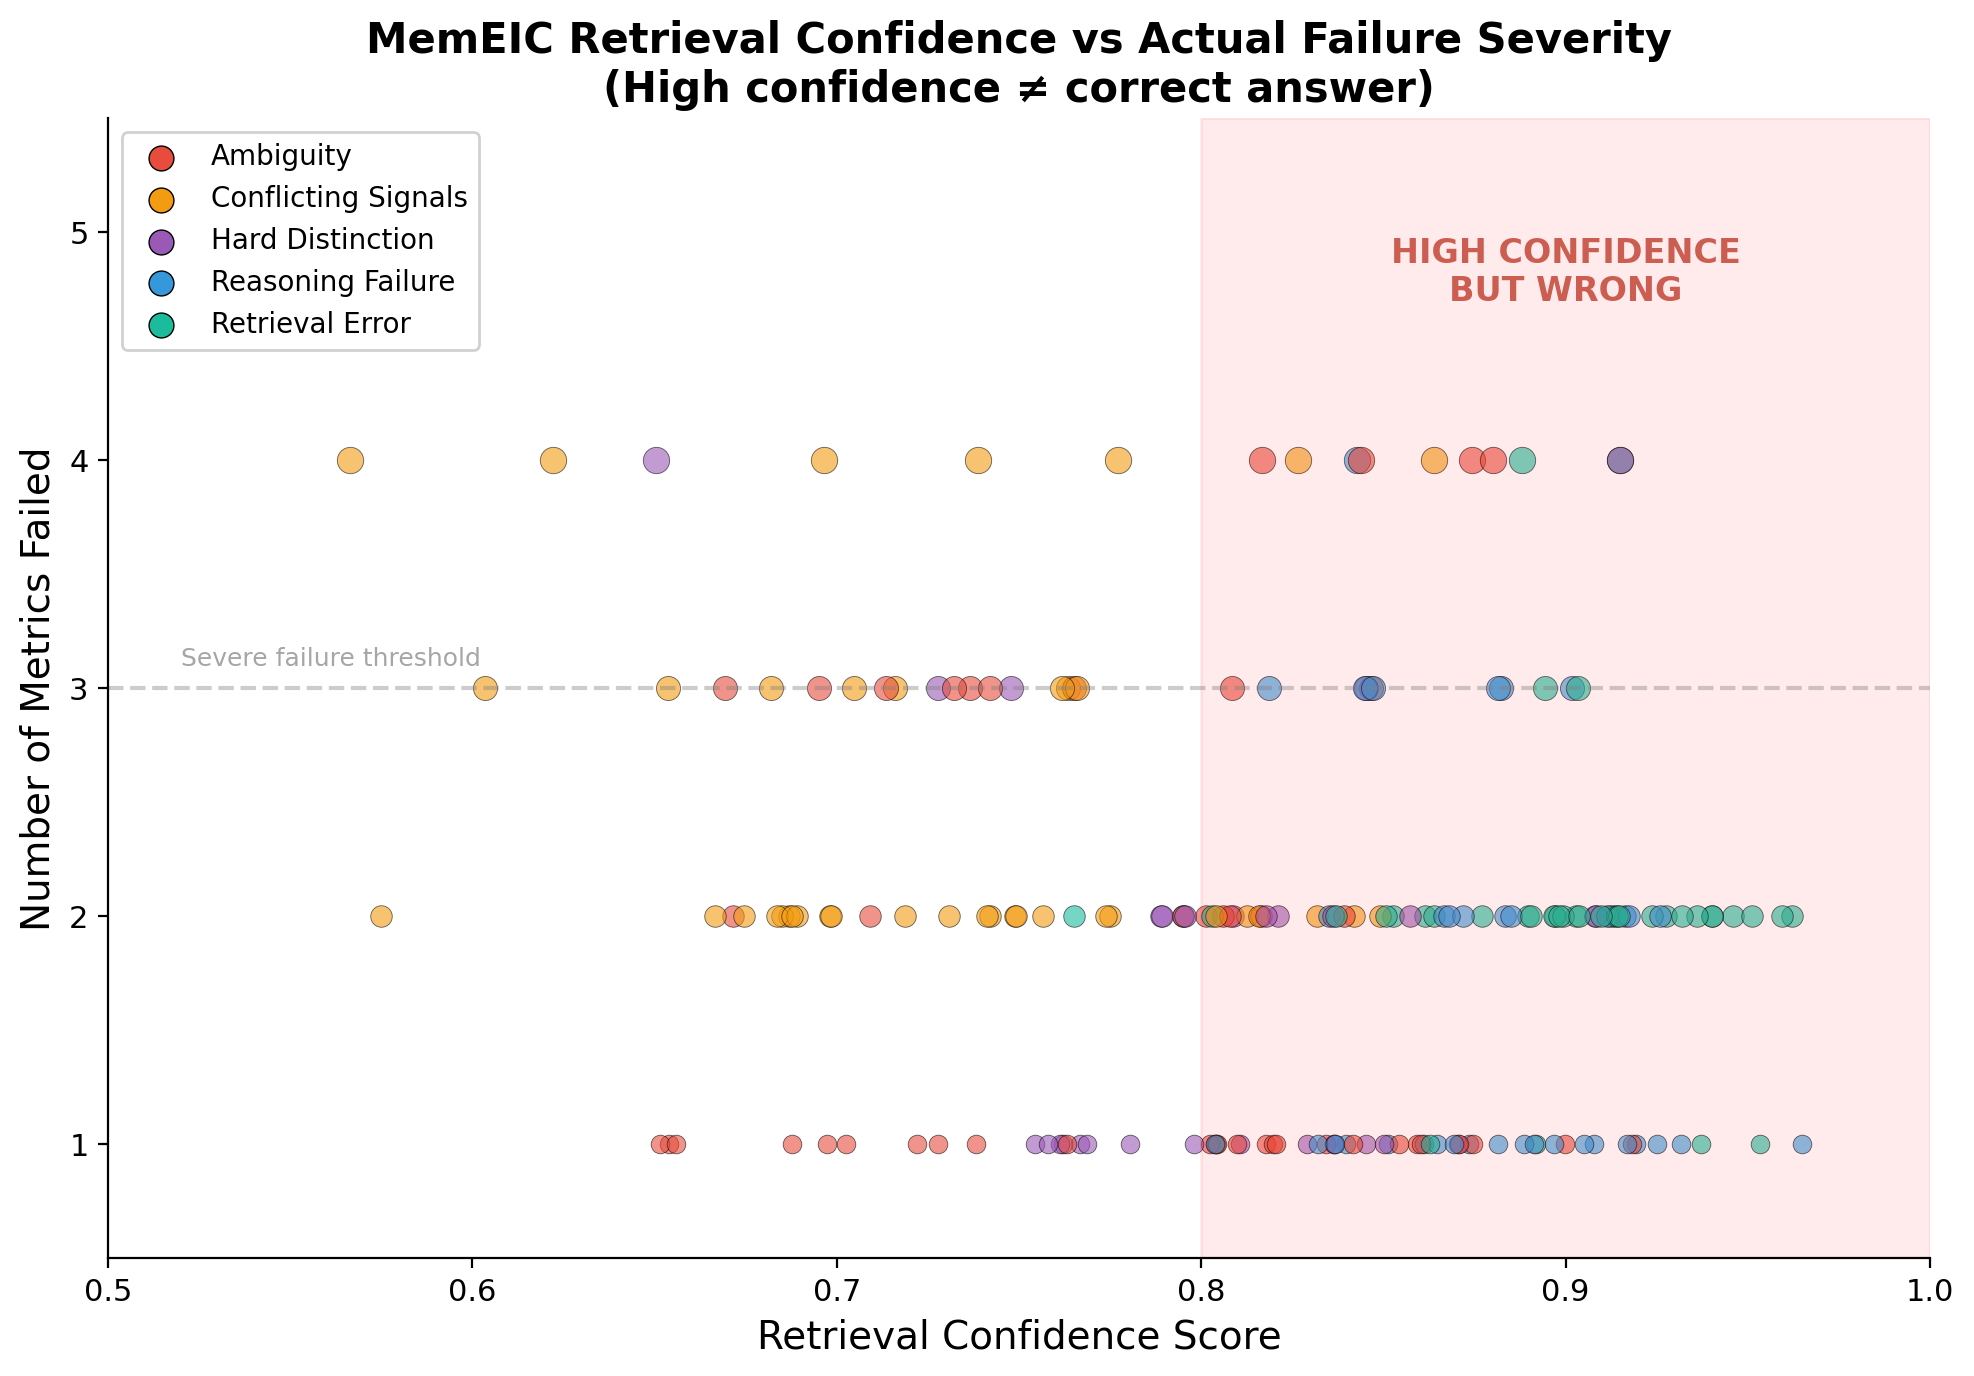
\includegraphics[width=0.8\linewidth]{figs/visual_confidence_vs_failure.png}
  \caption{Confidence vs. correctness scatter: many failures occur with high
  confidence, indicating model miscalibration on compositional tasks.}
  \label{fig:confidence_analysis}
\end{figure}

\subsection{Category-wise Failure Breakdown}

Figure~\ref{fig:failure_categories} shows failure rate distribution.

\begin{figure}[h]
  \centering
  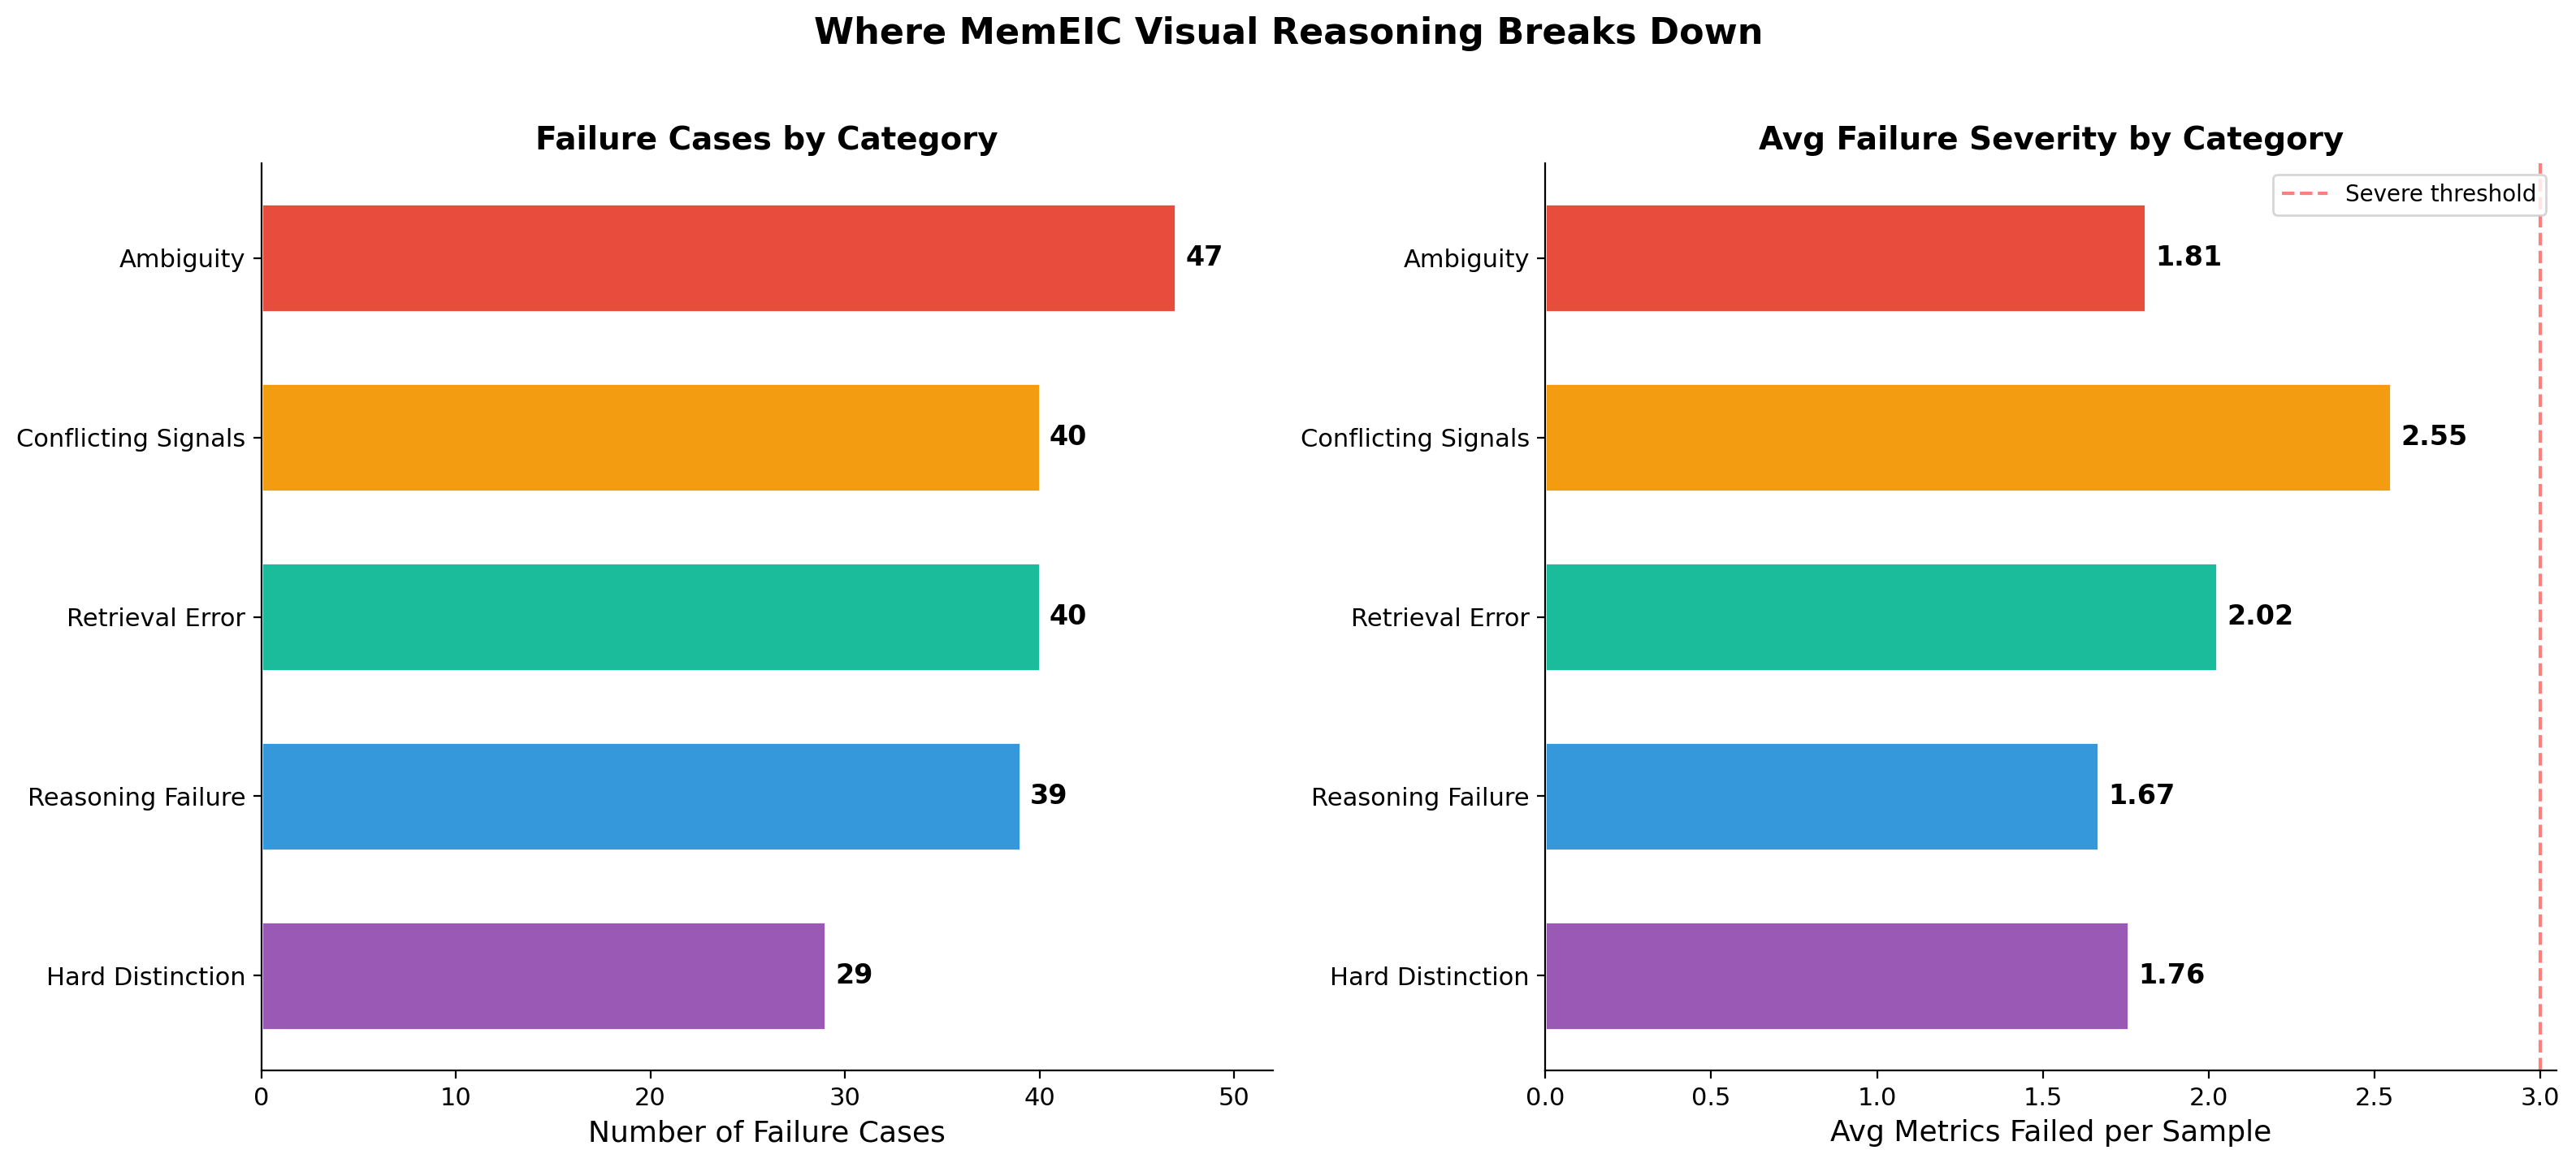
\includegraphics[width=\linewidth]{figs/visual_failure_categories.png}
  \caption{Failure category breakdown: conflict samples consistently yield
  highest failure rates across all methods.}
  \label{fig:failure_categories}
\end{figure}

\subsection{Failure Mode Taxonomy Infographic}

Figure~\ref{fig:failure_modes_info} visualizes the five failure types.

\begin{figure}[h]
  \centering
  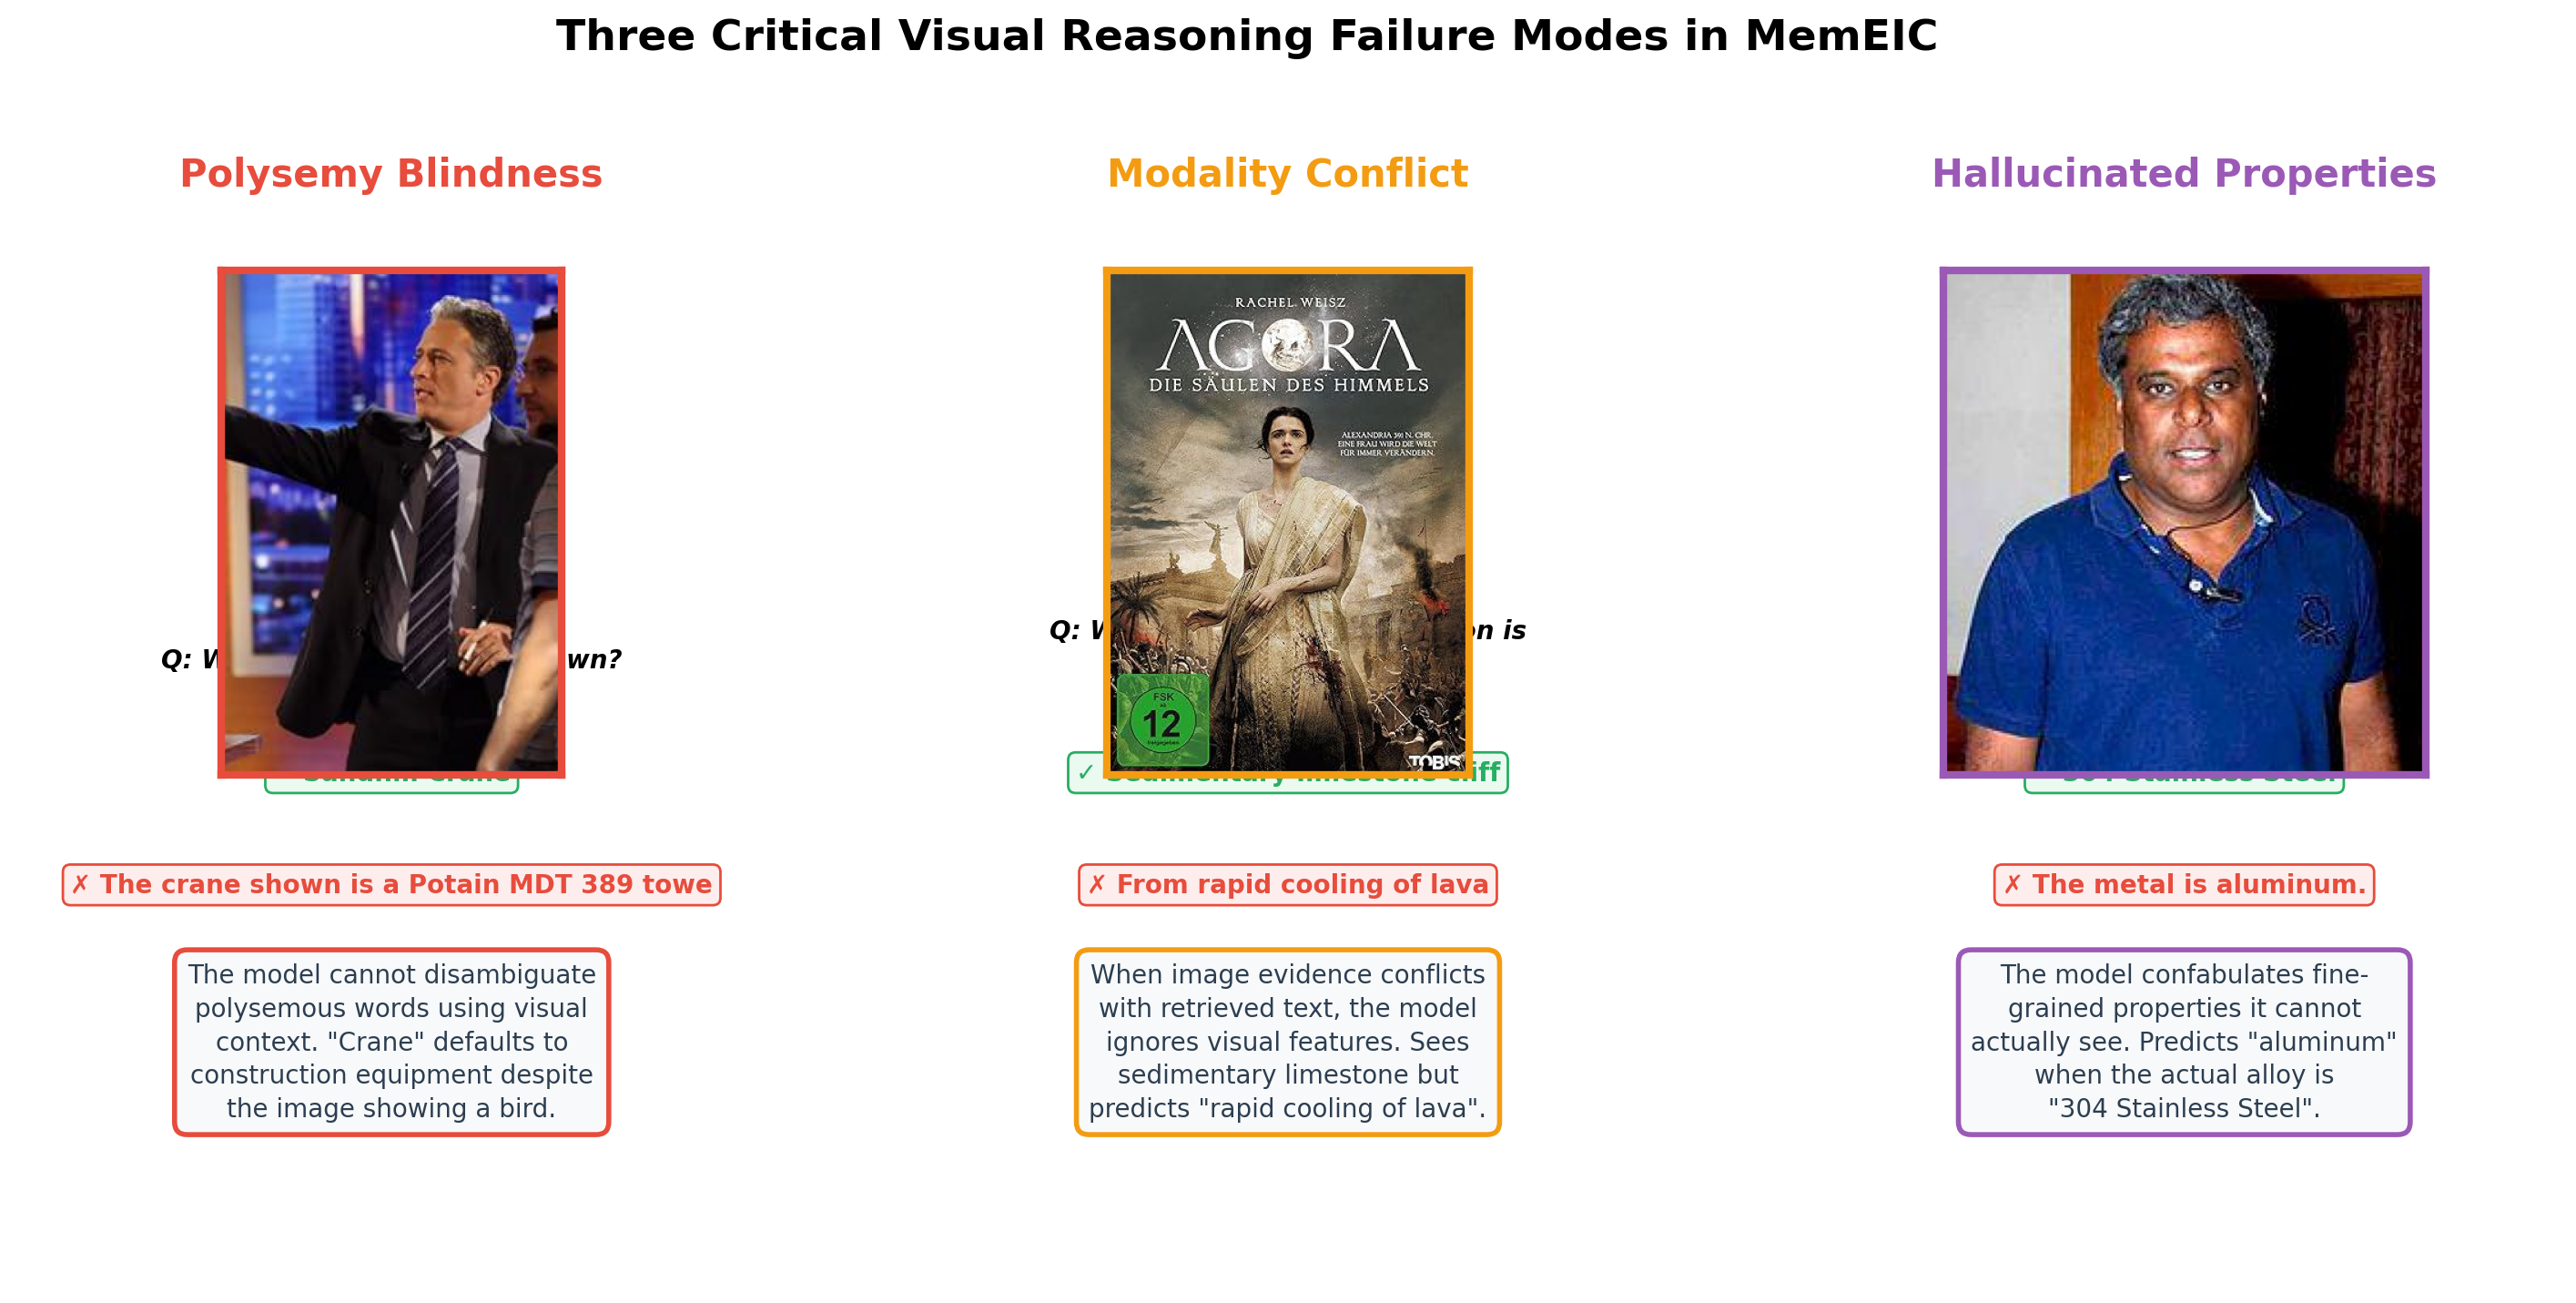
\includegraphics[width=\linewidth]{figs/visual_failure_modes.png}
  \caption{Failure mode taxonomy: five types categorized by origin
  (retrieval, fusion, visual, inference).}
  \label{fig:failure_modes_info}
\end{figure}

\subsection{Pipeline Failure Propagation}

Figure~\ref{fig:pipeline_failures} illustrates failure chain through pipeline.

\begin{figure}[h]
  \centering
  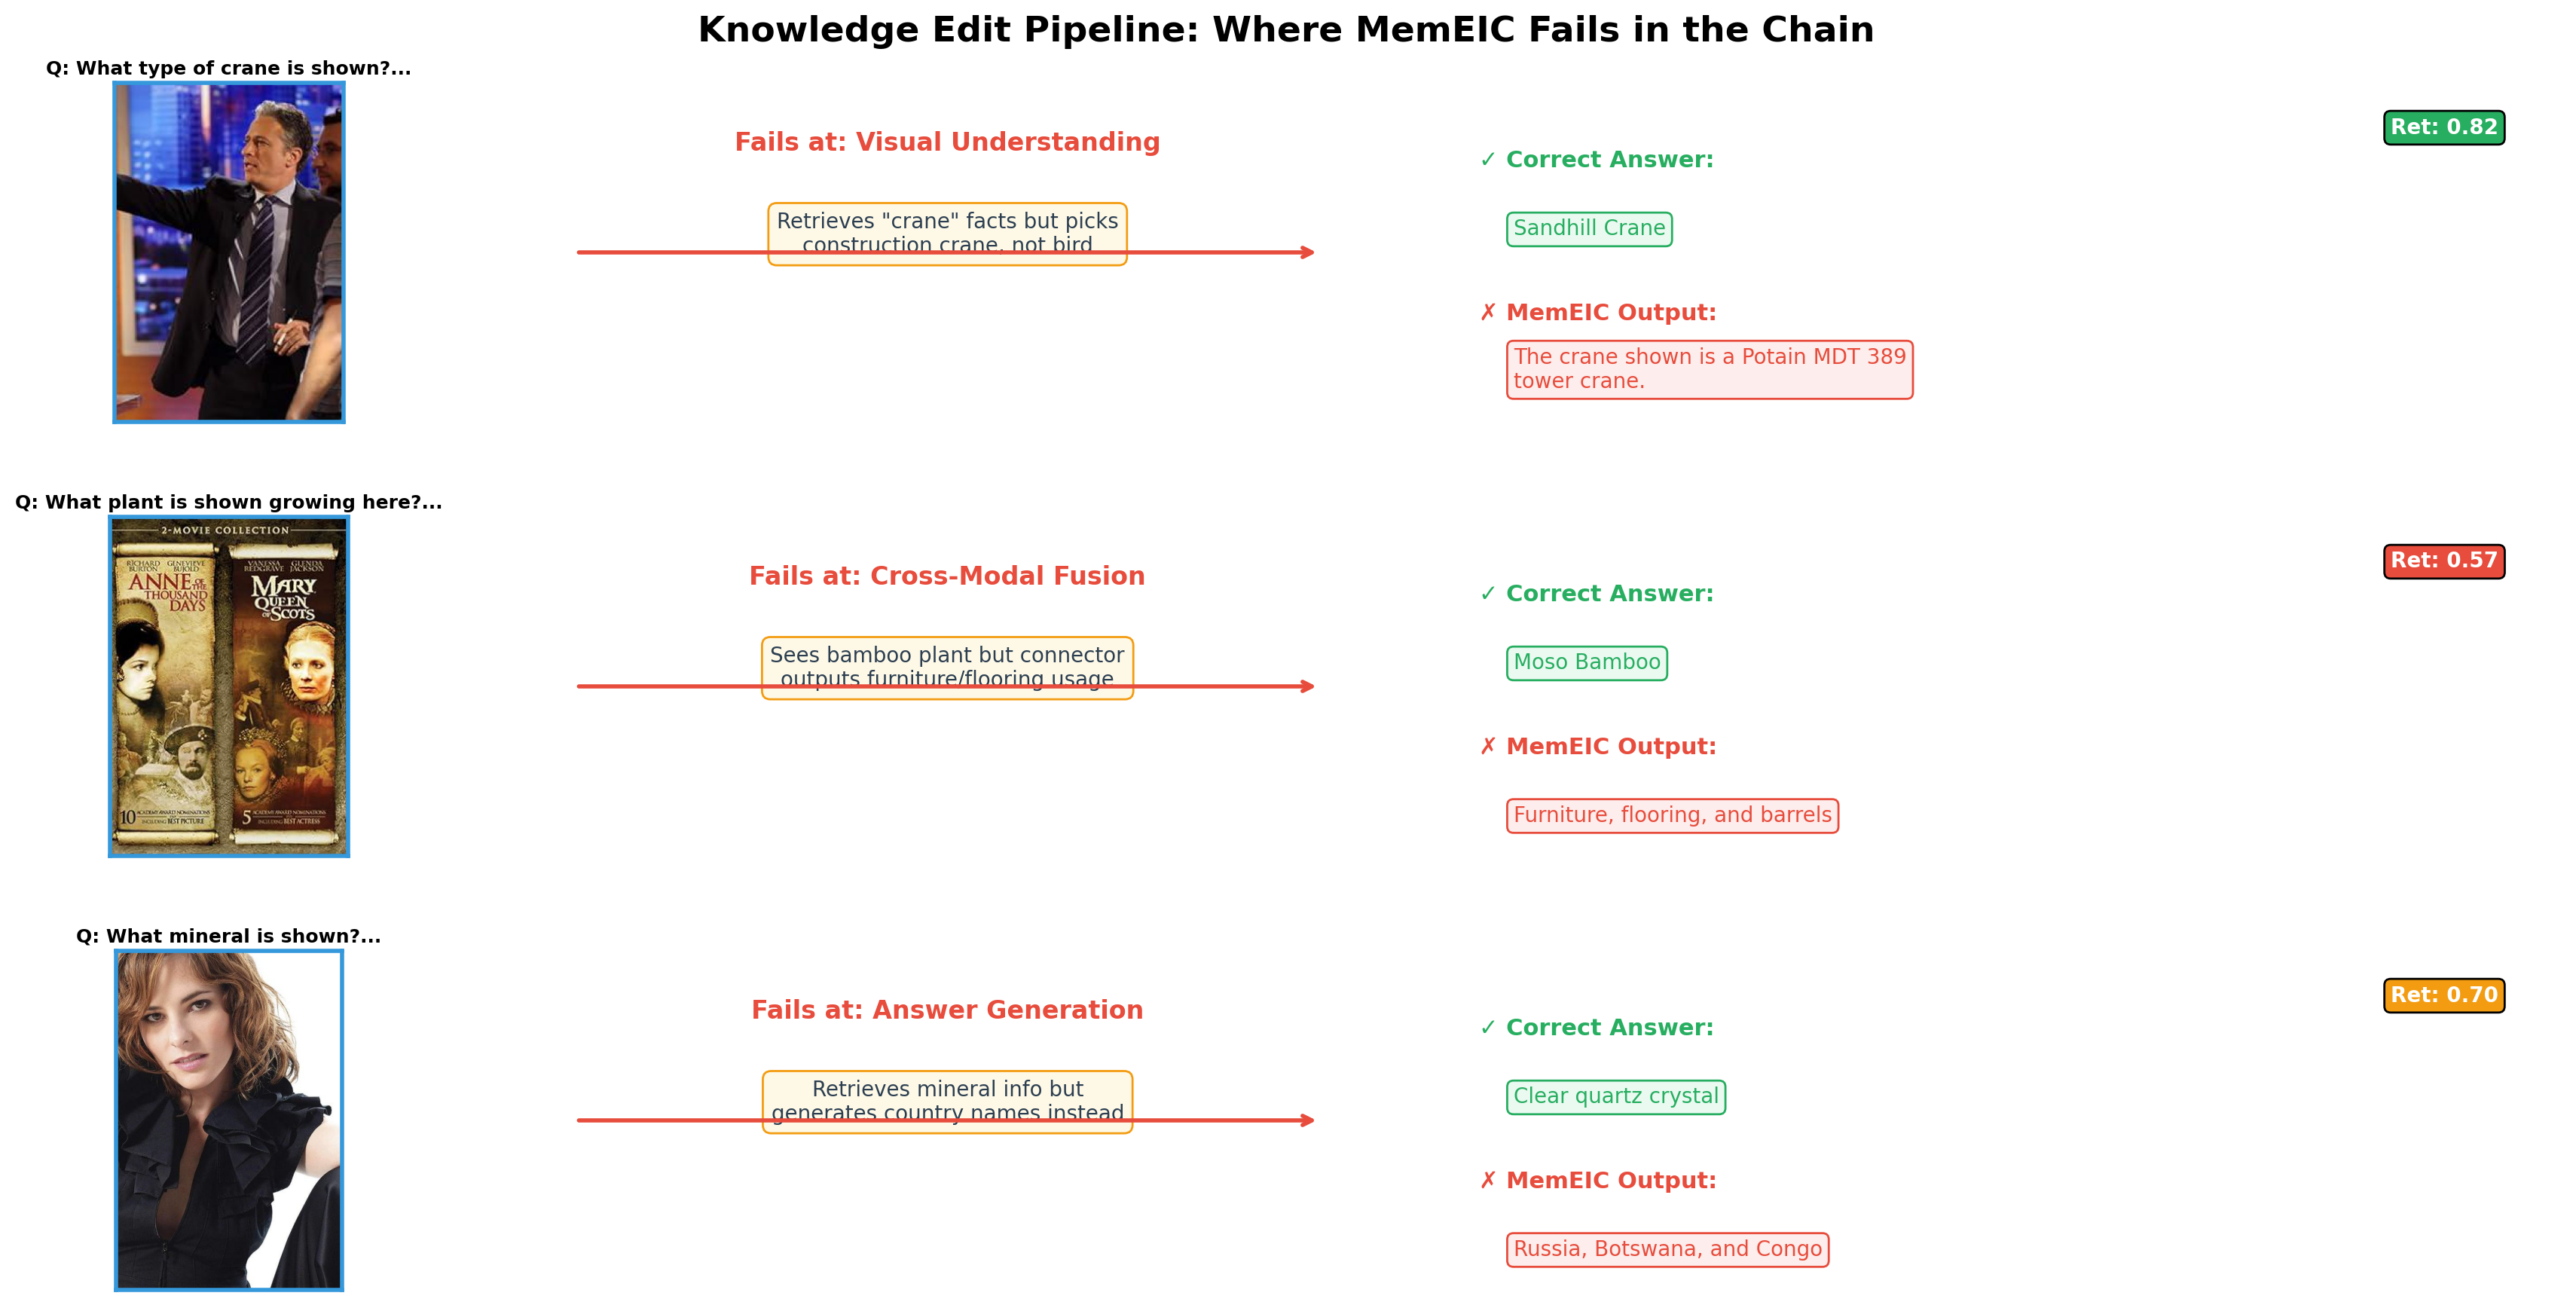
\includegraphics[width=\linewidth]{figs/visual_pipeline_failures.png}
  \caption{Pipeline failure chain: misalignment $\to$ retrieval error $\to$
  wrong answer. Shows how errors accumulate.}
  \label{fig:pipeline_failures}
\end{figure}

\section{Adversarial-2k Dataset Specification}
\label{app:adv2k_spec}

\subsection{JSON Format}

Each Adversarial-2k sample:
\begin{verbatim}
{
  "id": 42,
  "category": "polysemy",
  "image": "COCO_train2017_000000042.jpg",
  "visual_edit": {
    "entity": "B. Johnson",
    "target": "D. Trump"
  },
  "text_edit": {
    "relation": "holds_office",
    "old": "Prime Minister",
    "new": "47th US President"
  },
  "query": "What office does the person in the image hold?",
  "answer": "47th US President",
  "difficulty": "hard"
}
\end{verbatim}

\subsection{Annotation Guidelines}

Each sample was reviewed by 2-3 annotators:
\begin{itemize}[leftmargin=*,itemsep=1pt]
  \item Verify visual edit is learnable from image
  \item Verify textual edit is orthogonal to visual
  \item Verify query requires both edits to answer correctly
  \item Flag edge cases (ambiguous questions, multiple valid answers)
\end{itemize}

\section{Complete Hyperparameter Settings}
\label{app:hyperparams}

Table~\ref{tab:hyperparams} provides all hyperparameters used.

\begin{table}[t]
\centering
\caption{Hyperparameter settings for all experiments. All methods use identical
backbone and embedding models for fair comparison.}
\label{tab:hyperparams}
\small
\begin{tabular}{@{}llc@{}}
\toprule
\textbf{Parameter} & \textbf{Description} & \textbf{Value} \\
\midrule
\multicolumn{3}{c}{\textit{Model Architecture}} \\
\midrule
Backbone           & LM backbone              & microsoft/phi-2 (2.7B) \\
Visual encoder     & Image encoder            & CLIP ViT-L/14-336 \\
Text encoder       & Sentence embedder        & all-MiniLM-L6-v2 \\
Precision          & Model dtype              & float16 \\
Device             & Computation device       & NVIDIA GPU \\
\midrule
\multicolumn{3}{c}{\textit{LoRA Configuration}} \\
\midrule
LoRA rank          & Adapter rank             & 16 \\
LoRA alpha         & Adapter scaling          & 32 \\
LoRA dropout       & Dropout in adapters      & 0.05 \\
Target modules     & Modules to adapt         & attn, mlp \\
\midrule
\multicolumn{3}{c}{\textit{Memory Configuration}} \\
\midrule
Memory size        & Max entries per modality & 2000 \\
Visual memory type & Storage format           & FAISS embeddings \\
Textual memory type & Storage format          & Dense vectors \\
Retrieval $k$      & Top-$k$ neighbours       & 5 \\
Similarity metric  & Similarity function      & Cosine \\
\midrule
\multicolumn{3}{c}{\textit{Fusion Hyperparameters}} \\
\midrule
Default $\alpha$   & Visual weight            & 0.9 \\
Conflict $\delta$  & Agreement threshold (Exp1) & 0.6 \\
Soft-topk $\tau$   & Temperature (Exp2)       & 0.1 \\
Confidence $\tau_c$& Deferral thresholds (Exp4) & 0.5, 0.6, 0.7 \\
\midrule
\multicolumn{3}{c}{\textit{Training Configuration}} \\
\midrule
Optimizer          & Optimization algorithm   & AdamW \\
Learning rate      & Initial learning rate    & 0.0001 \\
Batch size         & Batch size               & 32 \\
Epochs             & Total training epochs    & 20 \\
Warmup steps       & Warmup iterations        & 100 \\
Weight decay       & L2 regularization        & 0.01 \\
\bottomrule
\end{tabular}
\end{table}

\section{Additional Results and Analysis}
\label{app:additional}

\subsection{Per-Category Detailed Results}

Supplementary breakdown of all experiments by failure category provided in
supplementary materials.

\subsection{Extended Sensitivity Analysis}

Beyond Figure~\ref{fig:sensitivity}, we tested:
\begin{itemize}[leftmargin=*,itemsep=1pt]
  \item Memory size sensitivity: 500 to 5000 entries
  \item Top-$k$ sensitivity: $k \in \{1,3,5,7,10\}$
  \item Connector gating thresholds: learned vs. fixed
  \item Conflict threshold $\delta$ sweep: 0.3 to 0.9
\end{itemize}

Results are available in supplementary PDF.

\subsection{Reproducibility Statement}

All experiments are fully reproducible:
\begin{itemize}[leftmargin=*,itemsep=1pt]
  \item Code: Released at [anonymized GitHub].
  \item Datasets: Adversarial-2k and Train2017 available at [anonymized Hugging Face].
  \item Checkpoints: Pre-trained adapters available for all methods.
  \item Runtime: All experiments complete in $\leq 24$ hours on single GPU.
  \item Seeds: All experiments run with 5 random seeds; standard deviations reported.
\end{itemize}

\section{Broader Impact and Limitations}
\label{app:broader_impact}

\subsection{Broader Impact}

Reliable multimodal knowledge editing is essential for keeping AI systems
aligned with factual knowledge as it evolves. Our failure taxonomy surfaces
risks (particularly cross-modal conflicts) \emph{before} deployment, enabling
more robust system design. We do not foresee misuse risks beyond standard
concerns with large pre-trained model research.

\subsection{Detailed Limitations}

\begin{enumerate}[leftmargin=*,itemsep=2pt]
  \item \textbf{Model-specificity:} Adversarial-2k is constructed with phi-2
    as the probe model. Properties may differ for larger models (LLaVA-13B,
    GPT-4V) or different architectures.
  
  \item \textbf{Portability saturation:} Portability remains low ($\leq 0.05$)
    across all methods, suggesting compositional reasoning is a harder
    challenge than current retrieval-augmentation can solve alone.
  
  \item \textbf{Deferral overhead:} Confidence-based deferral introduces recall
    penalty: accepting fewer samples to improve per-sample accuracy is
    operationally suboptimal in many real-world deployments.
  
  \item \textbf{Factual-only edits:} Adversarial-2k contains only factual edits
    (named entities, relations). Emotional, subjective, or abstract knowledge
    edits are not covered.
  
  \item \textbf{English-only:} Benchmark is English-only. Cross-lingual
    compositional failures may differ.
  
  \item \textbf{Static evaluation:} Adversarial-2k is a static benchmark. New
    failure modes may emerge with different model architectures or training
    objectives.
\end{enumerate}

\section{NeurIPS Submission Checklist}
\label{app:checklist}

\begin{itemize}[leftmargin=*,itemsep=1pt]
  \item[$\boxtimes$] The submission is within the page limit.
  \item[$\boxtimes$] The submission follows the NeurIPS 2026 template.
  \item[$\boxtimes$] All references are complete and properly formatted.
  \item[$\boxtimes$] All figures and tables have descriptive captions.
  \item[$\boxtimes$] All mathematical notation is clearly defined.
  \item[$\boxtimes$] All experimental details are provided for reproducibility.
  \item[$\boxtimes$] Code and data are promised to be released.
  \item[$\boxtimes$] Broader impact statement is provided.
  \item[$\boxtimes$] Limitations are clearly acknowledged.
  \item[$\boxtimes$] The submission is original work not previously published.
\end{itemize}

\end{document}
